\section{Struttura dei file}
	\subsection{Struttura del Json}
	I file Json che contengono la configurazione degli algoritmi di addestramento devono essere strutturati nei modi qui sotto indicati.
		\subsubsection{Regressione Lineare}
		\begin{itemize}
			\item \textbf{author} indica l'autore del file
			\item \textbf{version} indica la versione dell'applicazione con cui si è creato il file
			\item \textbf{date} indica la data in cui è stato creato il file
			\item \textbf{time} indica l'ora in cui è stato creato il file
			\item \textbf{pluginAim} indica l'algoritmo addestrato, in questo caso deve essere "rl"
			\item \textbf{predictors} elenco delle etichette dei predittori
			\item \textbf{result} elenco dei coefficienti risultati dall'addestramento
			\item \textbf{notes} eventuali note inserite durante l'addestramento
		\end{itemize}
		\mbox{}
		\begin{figure} [H]
			\begin{center}
				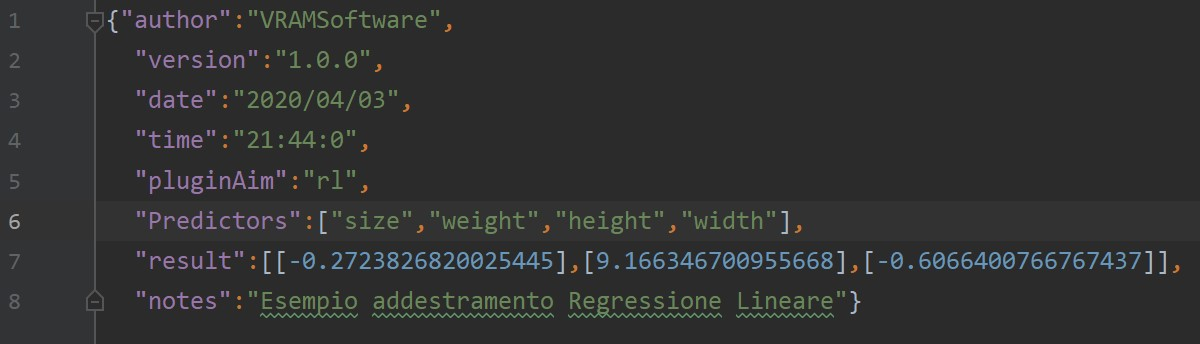
\includegraphics[width=\linewidth]{./img/jsonRl.jpg}
			\end{center}
			\caption{Esempio file Json per la Regressione Lineare}
		\end{figure}
		\mbox{}
		\subsubsection{Support Vector Machine}
			\begin{itemize}
				\item \textbf{author} indica l'autore del file
				\item \textbf{version} indica la versione dell'applicazione con cui si è creato il file
				\item \textbf{date} indica la data in cui è stato creato il file
				\item \textbf{time} indica l'ora in cui è stato creato il file
				\item \textbf{pluginAim} indica l'algoritmo addestrato, in questo caso deve essere "svm"
				\item \textbf{predictors} elenco delle etichette dei predittori
				\item \textbf{trainData} elenco dei dati addestrati
				\item \textbf{trainLabels} elenco delle label dei dati addestrati
				\item \textbf{result} elenco dei parametri risultati dall'addestramento, in particolare 
				\begin{itemize}
					\item \textbf{N} indica il numero di dati addestrati
					\item \textbf{D} indica la dimensione dei dati addestrati
					\item \textbf{b} indica lo scalare risultato dall'addestramento
					\item \textbf{kernelType} indica il tipo di kernel utilizzato, attualmente è implementato solo il kernel "linear"
					\item \textbf{w} indica il vettore risultato dall'addestramento					
				\end{itemize}
				\item \textbf{notes} eventuali note inserite durante l'addestramento
			\end{itemize}
		\mbox{}
		\begin{figure} [H]
			\begin{center}
				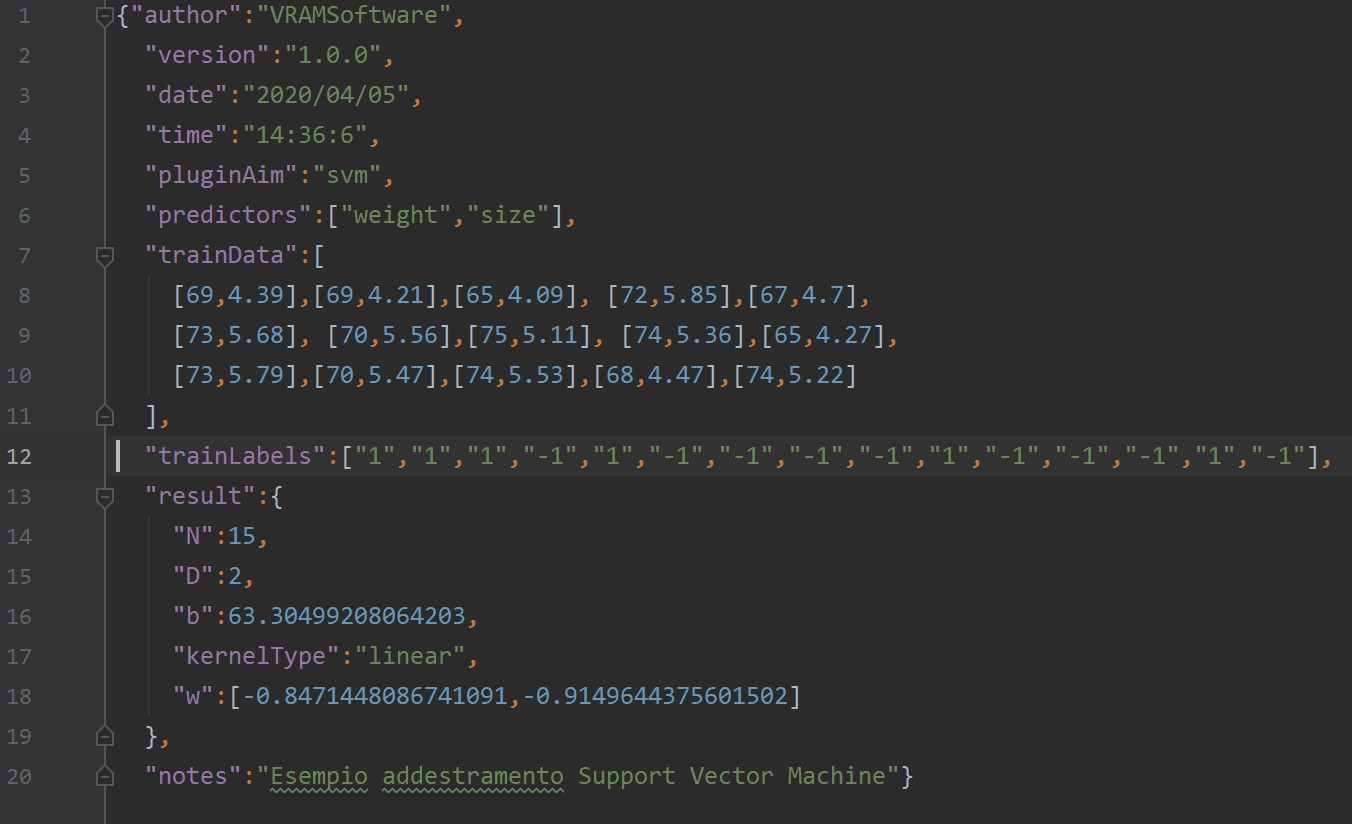
\includegraphics[width=\linewidth]{./img/jsonSvm.jpg}
			\end{center}
			\caption{Esempio file Json per la Support Vector Machine}
		\end{figure}
		\mbox{} \\ \\ 
		Se si desiderano ulteriori informazioni sulle regole sintattiche dei file JSON, si consiglia di consultare la documentazione W3C disponibile al seguente link:
		\\[0.2cm]
		\hspace*{10mm}
		\url{https://www.w3schools.com/js/js_json_syntax.asp}
		
	\subsection{Struttura del CSV}
	La struttura del file .csv è indipendente dall'algoritmo che si vuole addestrare.
	Deve presentare i valori di ogni predittore divisi per colonne, la prima riga di ogni colonna deve indicare l'etichetta associata al predittore. \\
	A seconda del caso devono essere presenti una o più colonne per i predetti, la prima riga di ogni colonna deve indicare l'etichetta associata al predetto.
	\mbox{}
	\begin{figure} [H]
		\begin{center}
			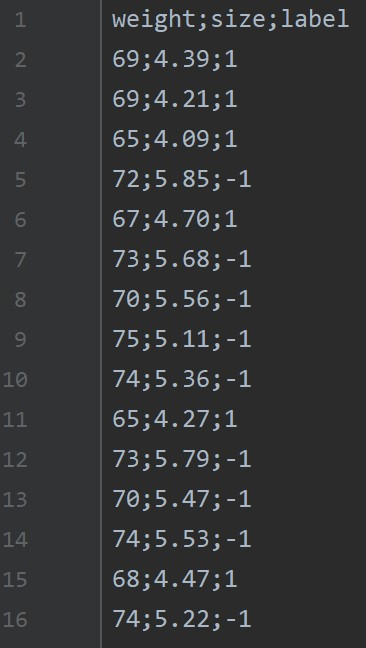
\includegraphics[width=50mm]{./img/csv1.jpg}
		\end{center}
		\caption{Esempio file csv}
	\end{figure}
	\mbox{}
	I file .csv possono eventualmente essere gestiti tramite fogli di calcolo
	\mbox{}
	\begin{figure} [H]
		\begin{center}
			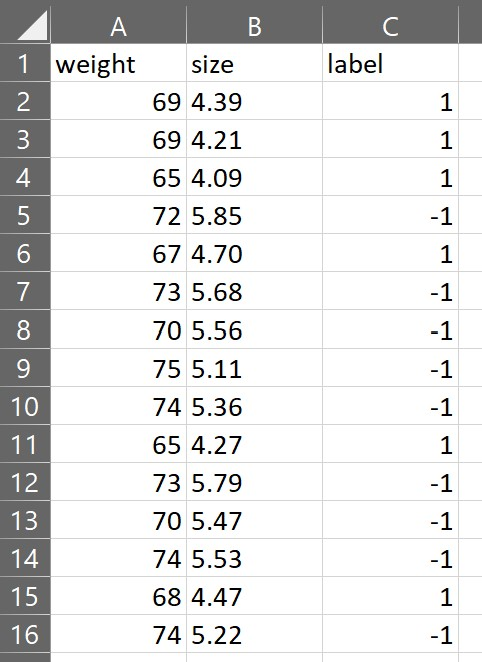
\includegraphics[width=50mm]{./img/csv2.jpg}
		\end{center}
		\caption{Esempio file csv su Microsoft Excel}
	\end{figure}
	\mbox{} 